\documentclass[11pt,a4paper]{article}

% ---------- Packages ----------
\usepackage[utf8]{inputenc}
\usepackage[T1]{fontenc}
\usepackage{lmodern}
\usepackage{amsmath,amssymb}
\usepackage{enumitem}
\usepackage{geometry}
\usepackage{fancyhdr}
\usepackage[most]{tcolorbox}   % enhanced, breakable
\usepackage{hyperref}

% ---------- Geometry ----------
\geometry{margin=2.5cm}

% ---------- Header/Footer ----------
\setlength{\headheight}{14pt}  % fancyhdr warning verhindern
\pagestyle{fancy}
\fancyhf{}
\lhead{Einführung in die Elektrotechnik}
\rhead{Wintersemester 2025}
\cfoot{\thepage}

% ---------- Exercise Environment ----------
\newcounter{exercise}
\newenvironment{exercise}[1][]
  {\refstepcounter{exercise}%
   \begin{tcolorbox}[enhanced, breakable, width=\textwidth,
     colback=blue!5!white,colframe=blue!60!black,
     fonttitle=\bfseries\large,
     title=Aufgabe~\theexercise:~#1]}
  {\end{tcolorbox}}

% ---------- Solution Environment ----------
\newif\ifshowsolutions
\showsolutionstrue  % comment to hide solutions

\newenvironment{solution}
  {\ifshowsolutions
     \begin{tcolorbox}[enhanced, breakable, width=\textwidth,
       colback=green!5!white,colframe=green!50!black,
       fonttitle=\bfseries\large,
       title=Lösung]}
  {\end{tcolorbox}\fi}

% ---------- Document ----------
\begin{document}

% ----- Header Box -----
\begin{tcolorbox}[enhanced, breakable, colback=gray!10!white,
  colframe=gray!70!black, fonttitle=\bfseries\large,
  title={Aufgabenblatt \#8}: Wechselstromschaltungen, sharp corners, width=\textwidth]
\begin{center}
  Besprechung: 08.12.2025
\end{center}
\end{tcolorbox}
\vspace{1cm}

% ----- Exercise 1 -----
\begin{exercise}[$RLC$ Stromkreis]
Bestimme $v(t)$ in der untenstehenden Schaltung.

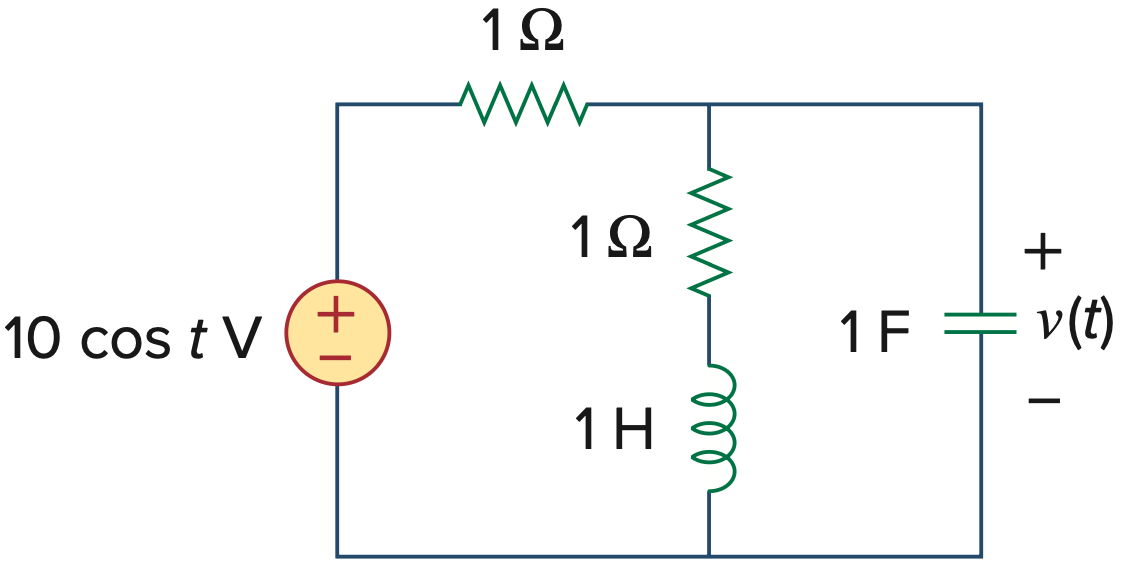
\includegraphics[width=0.7\textwidth]{figures/ACcircuit1.png}
\end{exercise}

\ifshowsolutions
\begin{solution}
Gegeben ist die zeitabhängige Spannungsquelle
\[
v_s(t) = 10\cos t\,\text{V}.
\]
In komplexer (exponentieller) Darstellung schreiben wir dies als Realteil einer komplexen Exponentialfunktion:
\[
v_s(t) = Re(\underline{\hat{v}}_s e^{j\omega t}),\qquad \underline{\hat{v}}_s = 10,\ \omega=1\ \text{rad/s},
\]
also \(v_s(t)=Re(10 e^{j t})\).

Für \(\omega=1\),
\[
\underline{Z}_{R_1} = 1,\qquad \underline{Z}_{R_2} = 1,\qquad \underline{Z}_L = j\omega L = j,\qquad \underline{Z}_C = \frac{1}{j\omega C} = -j.
\]

Die Reihenschaltung von \(R_2\) und \(L\) hat die Impedanz
\[
\underline{Z}_{RL}=1+j.
\]

Die Parallelschaltung von \(\underline{Z}_{RL}\) und \(\underline{Z}_C\) hat die Admittanz
\[
\underline{Y}_{p} = \frac{1}{\underline{Z}_{RL}} + \frac{1}{\underline{Z}_C} = \frac{1}{1+j} + \frac{1}{-j}.
\]
Berechnung der einzelnen Terme:
\[
\frac{1}{1+j} = \frac{1-j}{(1+j)(1-j)} = \frac{1-j}{2} = \tfrac12 - \tfrac12 j,
\qquad
\frac{1}{-j} = j.
\]
Somit ist
\[
\underline{Y}_p = \left(\tfrac12 - \tfrac12 j\right) + j = \tfrac12 + \tfrac12 j.
\]
Demnach ist die äquivalente Impedanz des Parallelnetzwerks
\[
\underline{Z}_p = \frac{1}{\underline{Y}_p} = \frac{1}{\tfrac12 + \tfrac12 j} = \frac{\tfrac12 - \tfrac12 j}{(\tfrac12)^2 + (\tfrac12)^2} = 1-j.
\]

Die gesamte Serienimpedanz, die die Quelle sieht, ist
\[
\underline{Z}_{\text{tot}} = \underline{Z}_{R_1} + \underline{Z}_p = 1+(1-j) = 2-j.
\]

Nun bilden wir den komplexen Strom \(\underline{\hat{i}}\) (die komplexe Amplitude, die mit \(e^{j t}\) multipliziert wird) durch Division der komplexen Quellamplitude durch die komplexe Impedanz:
\[
\underline{\hat{i}} = \frac{\underline{\hat{v}}_s}{\underline{Z}_{\text{tot}}} = \frac{10}{2-j}.
\]
Ausführen der Division durch Multiplikation von Zähler und Nenner mit dem konjugierten Wert des Nenners:
\[
\underline{\hat{i}} = 10\frac{2+j}{(2-j)(2+j)} = 10\frac{2+j}{5} = 4+2j.
\]
Demnach ist der komplexe Strom \(\underline{\hat{i}} = 4+2j\). (Der Betrag des Stromes ist \(|\underline{\hat{i}}| = \sqrt{4^2+2^2} \approx 4.472\) und sein Winkel \(\arg(\underline{\hat{i}}) = \arctan(2/4) = 26.57^\circ\), falls man Polardarstellung bevorzugt.)

Die komplexe Spannung über dem Parallelnetzwerk (und damit über dem Kondensator) ist
\[
\underline{\hat{v}}_p = \underline{\hat{i}}\,\underline{Z}_p = (4+2j)(1-j).
\]
Ausmultiplizieren:
\[
\underline{\hat{v}}_p = 4(1-j)+2j(1-j) = 4-4j+2j-2j^2 = 4-2j+2 = 6-2j.
\]
Die komplexe Spannung über dem Kondensator ist also \(\underline{\hat{v}}_p = 6-2j\).

Wir können dies auf zwei Arten ausdrücken:

\textbf{(a) Realteil der Exponentialfunktion im Zeitbereich:}
\[
v(t) = Re(\underline{\hat{v}}_p e^{j t}) = Re((6-2j)e^{j t}).
\]
Ausschreiben von \((6-2j)(\cos t + j\sin t)\) und Bestimmen des Realteils ergibt
\[
v(t) = 6\cos t + 2\sin t.
\]

\textbf{(b) Amplitude-Phasen-Form:} Berechnung von Betrag und Winkel von \(\underline{\hat{v}}_p\):
\[
|\underline{\hat{v}}_p| = \sqrt{6^2+(-2)^2} \approx 6.325,
\]
\[
\arg(\underline{\hat{v}}_p) = \arctan\!\bigg(\frac{-2}{6}\bigg) \approx -18.43^\circ.
\]
Somit ist
\[
\underline{\hat{v}}_p = 6.325\angle(-18.43^\circ),
\]
und demnach
\[
v(t) = 6.325\cos\big(t-18.43^\circ\big)\,\text{V},
\]
was algebraisch äquivalent zu \(v(t) = 6\cos t + 2\sin t\) ist.
\end{solution}
\fi

% ----- Exercise 2 -----
\begin{exercise}[Phasenverschobener Quellenstrom]
Bestimme den Quellenstrom $i_s(t)$ in der untenstehenden Schaltung.

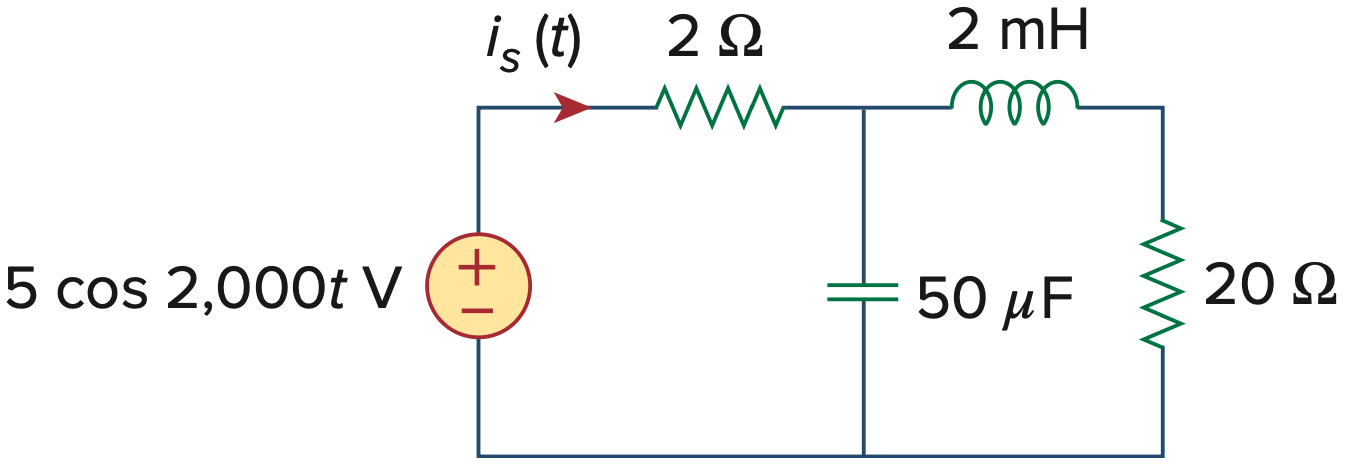
\includegraphics[width=0.7\textwidth]{figures/ACcircuit2.png}
\end{exercise}

\ifshowsolutions
\begin{solution}
\[
\omega = 2000\;\text{rad/s}
\]

\[
\underline{Z}_C = \frac{1}{j \omega C} = \frac{-j}{2000 \cdot 50 \times 10^{-6}}\,\Omega = -j 10\,\Omega
\]

\[
\underline{Z}_{RL} = 20 + j \omega L = (20 + j 2000 \cdot 2 \times 10^{-3})\,\Omega = (20 + j 4)\,\Omega
\]

\[
\underline{Y}_p = \frac{1}{\underline{Z}_C} + \frac{1}{Z_{RL}} = j 0.1 + \frac{1}{20 + j 4} = j 0.1 + \frac{20 - j 4}{416} = \left(\frac{20}{416} + j \frac{37.6}{416}\right)\,\text{S}
\]

\[
\underline{Z}_p = \frac{1}{\underline{Y}_p} = \left(\frac{\frac{20}{416} - j \frac{37.6}{416}}{(\frac{20}{416})^2 + (\frac{37.6}{416})^2}\right)\,\Omega = (4.58716 - j 8.62385)\,\Omega
\]

\[
\underline{Z}_{\text{tot}} = \underline{Z}_{R_2} + Z_p = 2\,\Omega + (4.58716 - j8.62385)\,\Omega = (6.58716 - j 8.62385)\,\Omega
\]

\[
\underline{\hat{i}}_s = \frac{\underline{\hat{v}}_s}{\underline{Z}_{\text{tot}}} = \frac{5}{6.58716 - j 8.62385}\,\text{A} = (0.27714 + j 0.36949)\,\text{A}
\]

\[
\hat{i}_s = \sqrt{(0.27714)^2 + (0.36949)^2}\,\text{A} = 0.460753\,\text{A}
\]

\[
\varphi_{i_s} = \tan^{-1}\!\left(\frac{0.36949}{0.27714}\right) = 52.6263^\circ
\]

\[
i_s(t) = 460.7 \cos\!\left(2000t + 52.63^\circ\right)\,\text{mA}
\]
\end{solution}
\fi

% ----- Exercise 3 -----
\begin{exercise}[Äquivalenzimpedanz]
Bestimme die Äquivalenzimpedanz $\underline{Z}_{eq}$ in der untenstehenden Schaltung.

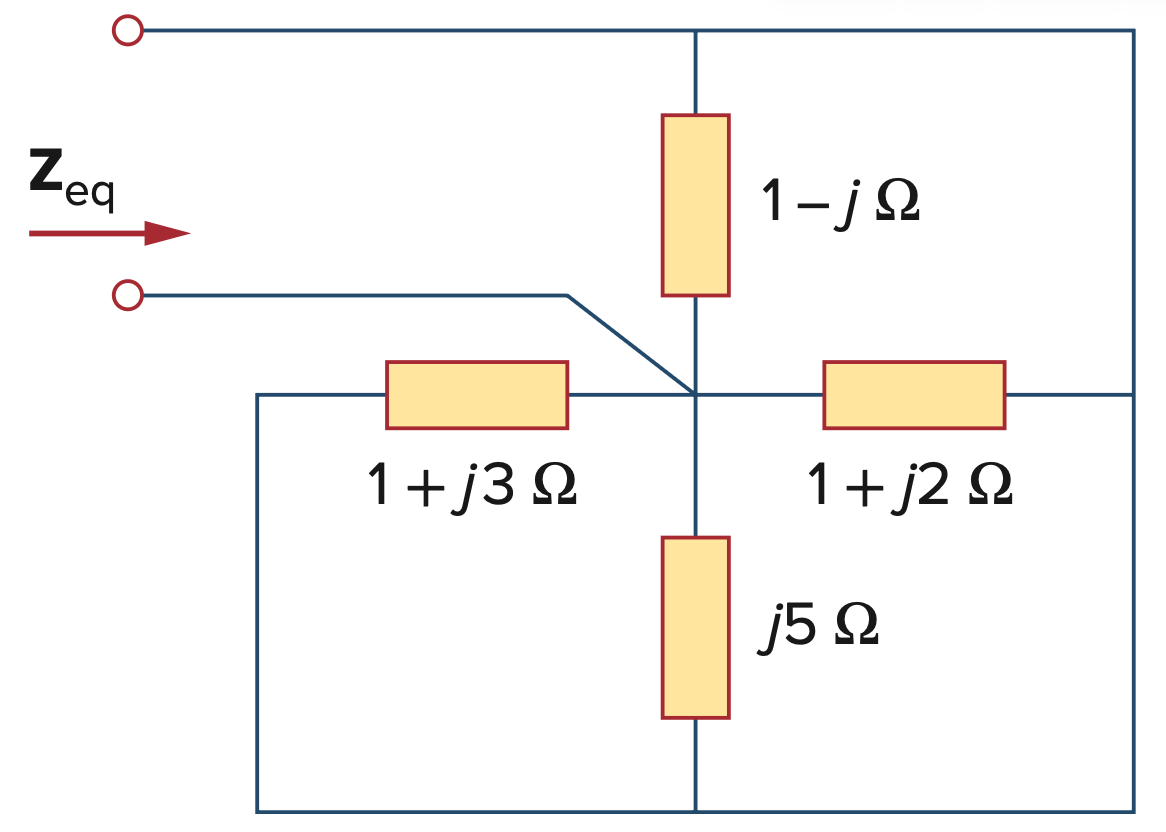
\includegraphics[width=0.7\textwidth]{figures/ACcircuit3.png}
\end{exercise}

\ifshowsolutions
\begin{solution}
\[
\underline{Y} = \frac{1}{\underline{Z}_1} + \frac{1}{\underline{Z}_2} + \frac{1}{\underline{Z}_3} + \frac{1}{\underline{Z}_4} = \frac{1}{1 - j} + \frac{1}{1 + j 2} + \frac{1}{1 + j 3} + \frac{1}{j 5}
\]
\[
= \frac{1 + j}{2} + \frac{1 - j 2}{5} + \frac{1 - j 3}{10} + \frac{-j 5}{25} = \frac{25 + 10 + 5 + j (25 - 20 - 15 - 10)}{50} = (0.8 - j 0.4)\,\text{S}
\]

\[
\underline{Z}_{eq} = \frac{1}{\underline{Y}} = \frac{1}{0.8 - j 0.4} = \frac{0.8 + j 0.4}{0.8^2 + 0.4^2} = (1 + j 0.5)\,\Omega
\]
\end{solution}
\fi

% ----- Exercise 4 -----
\begin{exercise}[Schrittweise Spannungsteilung]
\begin{enumerate}[label=\alph*)]
  \item Berechne die Phasenverschiebung der untenstehenden Schaltung.
  \item Gib an ob die Phasenverschiebung vor- oder nachlaufend ist (Ausgang bezogen auf Eingang).
  \item Bestimme die Amplitude des Ausgangs, wenn der Eingang \(120\,\text{V}\) beträgt.
\end{enumerate}

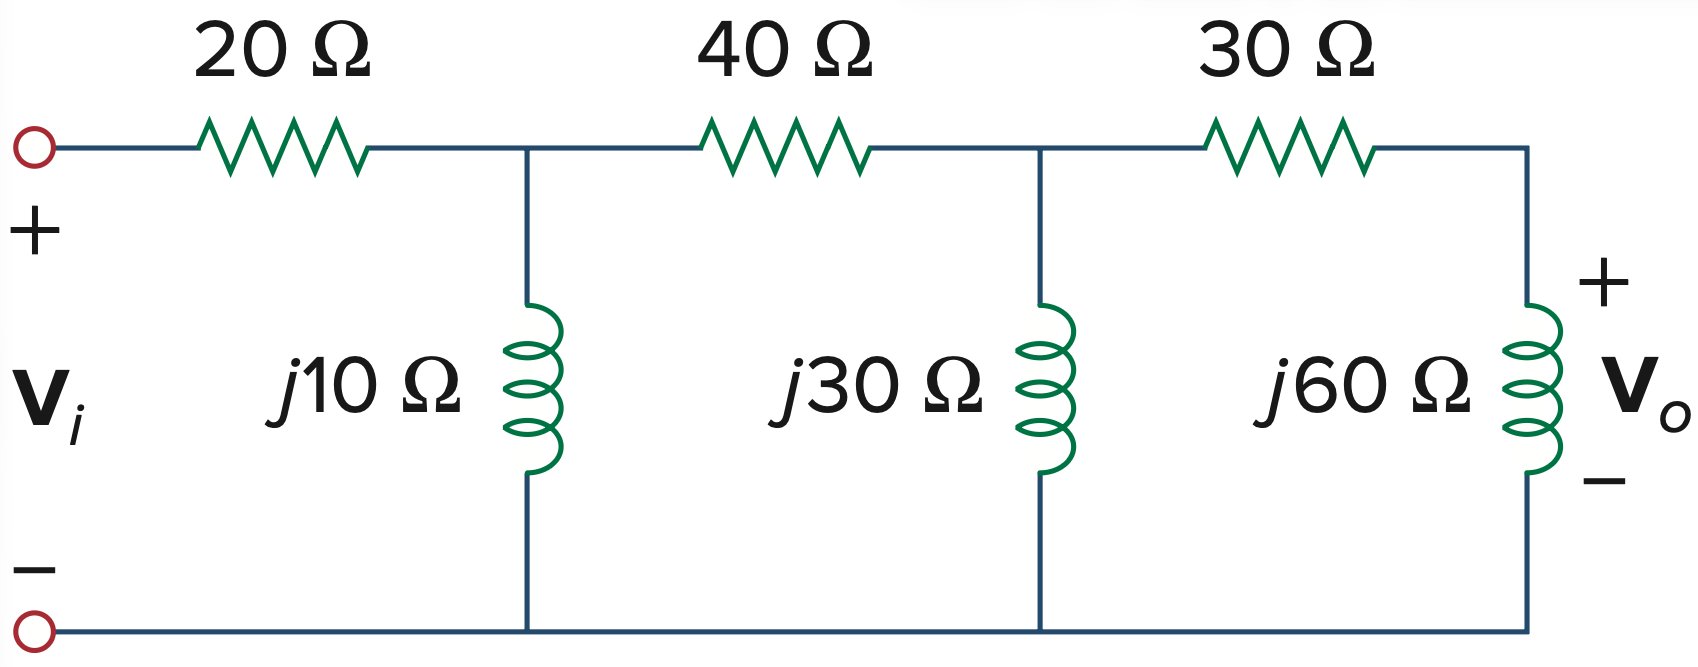
\includegraphics[width=0.7\textwidth]{figures/ACcircuit4.png}
\end{exercise}

\ifshowsolutions
\begin{solution}
\begin{enumerate}[label=\alph*)]
\item Wir nehmen die Eingangsspannung \(\underline{v}_i\) als Referenzphasor (Winkel \(0^\circ\)) und bezeichnen die Knotenspannungen mit \(\underline{v_1}, \underline{v_2}, \underline{v_3}\) (wobei \(\underline{v}_3 = \underline{v}_o\)).

Schritt 1: Relation zwischen \(\underline{v}_3\) und \(\underline{v}_2\)

Knoten 3 ist ein einfacher Spannungsteiler zwischen dem Serienwiderstand \(R_3\) und der Induktivität \(\underline{Z}_3\):
\[
\underline{v}_3 = \underline{v}_2 \cdot \frac{\underline{Z}_3}{R_3 + \underline{Z}_3}.
\]
Mit \(R_3 = 30,\; \underline{Z}_3 = j60\):
\[
\frac{\underline{v}_3}{\underline{v}_2} = \frac{j60}{30 + j60} = \frac{1}{1 - j 0.5} = 0.8 + 0.4\,j
\]
\[
= \sqrt{0.8^2 + 0.4^2} \cdot \exp\!\left(j \arctan\!\left(\frac{0.4}{0.8}\right)\right) = 0.894427 \cdot \exp(j 26.565^\circ).
\]

Schritt 2: Äquivalenzimpedanz gesehen von Knoten 2

Knoten 2 sieht \(\underline{Z}_2\) parallel zur Reihenschaltung von \(R_3\) und \(\underline{Z}_3\):
\[
\underline{Z}_{\text{eq2}} = \frac{\underline{Z}_2 (R_3 + \underline{Z}_3)}{\underline{Z}_2 + (R_3 + \underline{Z}_3)}.
\]
Mit \(\underline{Z}_2 = j30\):
\[
R_3 + \underline{Z}_3 = 30 + j60,
\]
\[
\underline{Z}_{\text{eq2}} = \frac{j30 (30 + j60)}{j30 + (30 + j60)} = \frac{j900 - 1800}{30 + j90} = \frac{27000 + j189000}{9000} = 3 + j21.
\]

Nun wenden wir den Teiler zwischen \(R_2\) und \(\underline{Z}_{\text{eq2}}\) an:
\[
\underline{v}_2 = \underline{v}_1 \cdot \frac{\underline{Z}_{\text{eq2}}}{R_2 + \underline{Z}_{\text{eq2}}}.
\]
\[
\frac{\underline{v}_2}{\underline{v}_1} = \frac{3 + j21}{40 + 3 + j21} = \frac{(3 + j21) (43 - j21)}{43^2 + 21^2} = \frac{57 + j84}{229}
\]
\[
= \frac{\sqrt{57^2 + 84^2}}{229} \cdot \exp\!\left(j \arctan\!\left(\frac{84}{57}\right)\right) = 0.443291 \cdot \exp\!\left(j 55.840^\circ\right).
\]

Schritt 3: Äquivalenzimpedanz gesehen von Knoten 1

Knoten 1 sieht \(\underline{Z}_1\) parallel zur Reihenschaltung von \(R_2\) und \(\underline{Z}_{\text{eq2}}\):
\[
\underline{Z}_{\text{eq1}} = \frac{\underline{Z}_1 (R_2 + \underline{Z}_{\text{eq2}})}{\underline{Z}_1 + (R_2 + \underline{Z}_{\text{eq2}})}
\]

\[
R_2 + \underline{Z}_{\text{eq2}} = 40 + 3 + j21 = 43 + j21,
\]
\[
\underline{Z}_1 (R_2 + \underline{Z}_{\text{eq2}}) = j10 (43 + j21) = -210 + j430
\]
\[
\underline{Z}_1 + (R_2 + \underline{Z}_{\text{eq2}}) = j10 + (43 + j21) = 43 + j31
\]
Somit ist
\[
\underline{Z}_{\text{eq1}} = \frac{-210 + j430}{43 + j31} = \frac{(-210 + j430)(43 - j31)}{43^2 + 31^2} = \frac{4300 + j25000}{2810}
\]
\[
= \sqrt(4300^2 + 25000^2) \cdot \exp\!\left(j \arctan\!\left(25000/4300\right)\right) \cdot \frac{1}{2810} = 9.027439 \cdot \exp\!\left(j 80.241^\circ\right).
\]

Dann gilt für den Teiler zwischen \(R_1\) und \(\underline{Z}_{\text{eq1}}\):
\[
\underline{v}_1 = \underline{v}_i \cdot \frac{\underline{Z}_{\text{eq1}}}{R_1 + \underline{Z}_{\text{eq1}}}.
\]
\[
R_1 + \underline{Z}_{\text{eq1}} = 20 + \frac{4300 + j25000}{2810} = \frac{20 \cdot 2810 + 4300 + j25000}{2810} = \frac{60500 + j25000}{2810}
\]
\[
= \sqrt(60500^2 + 25000^2) \cdot \exp\!\left(j \arctan\!\left(25000/60500\right)\right) \cdot \frac{1}{2810} = 23.296022 \cdot \exp\!\left(j 22.452^\circ\right)
\]
\[
\frac{\underline{v}_1}{\underline{v}_i} = \frac{9.027439}{23.296022} \cdot \exp\!\left(j (80.241^\circ - 22.452^\circ)\right) = 0.387510 \cdot \exp\!\left(j 57.789^\circ\right)
\]

Schritt 4: Kombination der drei Verhältnisse

Ausgang relativ zum Eingang:
\[
\frac{\underline{v}_o}{\underline{v}_i} = \frac{\underline{v}_3}{\underline{v}_i} = \frac{\underline{v}_3}{\underline{v}_2} \cdot\frac{\underline{v}_2}{\underline{v}_1} \cdot\frac{\underline{v}_1}{\underline{v}_i}
\]
\[
= 0.894427 \cdot \exp\!\left(j 26.565^\circ\right) \cdot 0.443291 \cdot \exp\!\left(j 55.840^\circ\right) \cdot 0.387510 \cdot \exp\!\left(j 57.789^\circ\right)
\]
\[
= 0.153644 \cdot \exp\!\left(j 140.194^\circ\right)
\]
\[
\Rightarrow \varphi = 140.2^\circ
\]

\item Da die Phasenverschiebung positiv ist (\(+140.2^\circ\)), läuft der Ausgangsphasor dem Eingangsphasor **vor**.

\item Größe des Ausgangs für \(V_i = 120\,\text{V}\):
\[
V_o = 0.153644 \cdot 120\,\text{V} \approx 18.44\,\text{V}
\]
\end{enumerate}
\end{solution}
\fi

% ----- Exercise 5 -----
\begin{exercise}[Knotenpotentialsanalyse]
Bestime den Strom $i$ in der untenstehenden Schaltung.

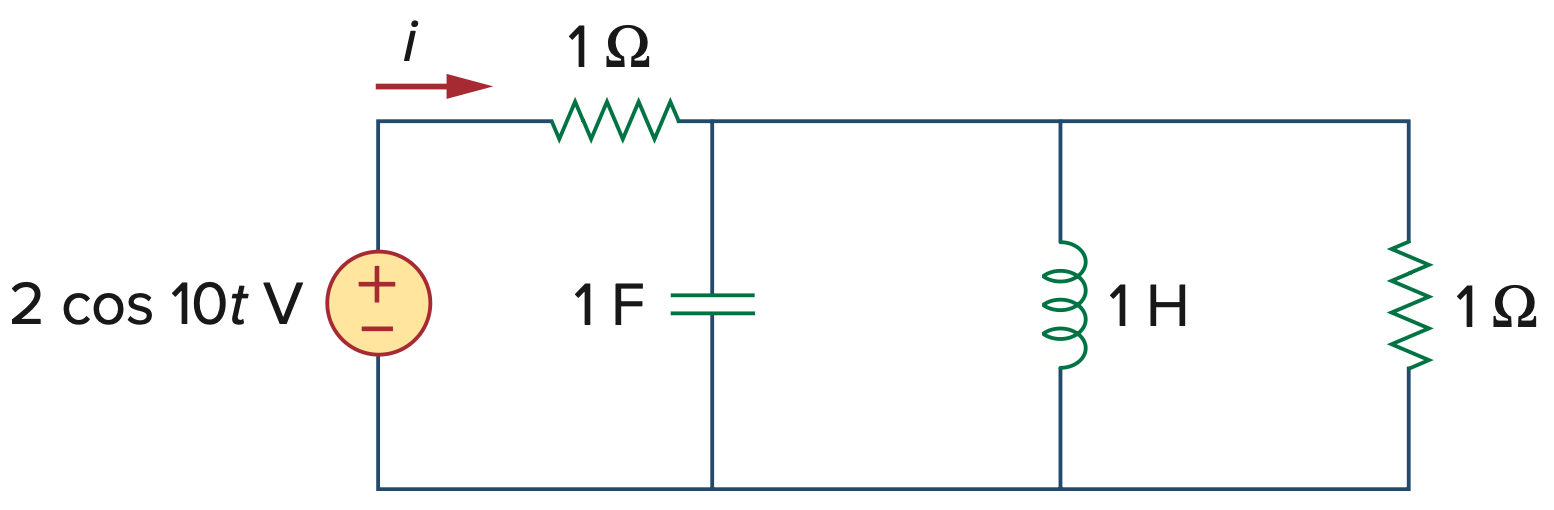
\includegraphics[width=0.7\textwidth]{figures/ACnodal.png}
\end{exercise}

\ifshowsolutions
\begin{solution}
\[
v_s(t) = 2\cos(10t)\quad\Rightarrow\quad \omega=10
\]
Kondensator- und Induktivitätsadmittanzen (1\,F und 1\,H):
\[
\underline{Y}_C = j\omega C = j10,\qquad \underline{Y}_L = \frac{1}{j\omega L} = -\frac{j}{10} = -j0.1,
\]
und der Parallelwiderstand liefert \(R = 1\). Somit ist die Gesamtadmittanz des Parallelnetzwerks
\[
\underline{Y} = R + \underline{Y}_C + \underline{Y}_L = 1 + j10 - j0.1 = 1 + j9.9.
\]

KCL an dem Knoten (Strom durch die Reihenschaltung \(1\Omega\) ist gleich dem Strom in das Parallelnetzwerk):
\[
\frac{\hat{v}_s - \underline{\hat{v}}}{1} = \underline{\hat{v}}\;\underline{Y}
\quad\Longrightarrow\quad
\underline{\hat{v}}\,(1 + \underline{Y}) = \hat{v}_s
\quad\Longrightarrow\quad
\underline{\hat{v}} = \frac{\hat{v}_s}{1 + \underline{Y}}.
\]
Der Quellstrom \( \underline{\hat{i}}\) (welcher im Zeitbereich \(i\) ist) ist der Strom durch den Serienwiderstand \(1\Omega\):
\[
\underline{\hat{i}} = \frac{\hat{v}_s - \underline{\hat{v}}}{1} = \hat{v}_s \frac{\underline{Y}}{1 + \underline{Y}}
\]

Einsetzen von \(\underline{Y} = 1 + j9.9\):
\[
\underline{\hat{i}} = 2 \cdot \frac{1 + j9.9}{2 + j9.9} = \frac{200.02 + j19.8}{102.01} \approx (1.9608 + j0.1941)\,\text{A}
\]

Amplitude, Phase und Rücktransformation in den Zeitbereich (Kosinus-Referenz):
\[
i(t) = 1.9704\cos\big(10t + 5.655^\circ\big)\,\text{A}
\]
\end{solution}
\fi

\end{document}